% Options for packages loaded elsewhere
\PassOptionsToPackage{unicode}{hyperref}
\PassOptionsToPackage{hyphens}{url}
%
\documentclass[
  ignorenonframetext,
  aspectratio=169]{beamer}
\usepackage{pgfpages}
\setbeamertemplate{caption}[numbered]
\setbeamertemplate{caption label separator}{: }
\setbeamercolor{caption name}{fg=normal text.fg}
\beamertemplatenavigationsymbolsempty
% Prevent slide breaks in the middle of a paragraph
\widowpenalties 1 10000
\raggedbottom
\setbeamertemplate{part page}{
  \centering
  \begin{beamercolorbox}[sep=16pt,center]{part title}
    \usebeamerfont{part title}\insertpart\par
  \end{beamercolorbox}
}
\setbeamertemplate{section page}{
  \centering
  \begin{beamercolorbox}[sep=12pt,center]{part title}
    \usebeamerfont{section title}\insertsection\par
  \end{beamercolorbox}
}
\setbeamertemplate{subsection page}{
  \centering
  \begin{beamercolorbox}[sep=8pt,center]{part title}
    \usebeamerfont{subsection title}\insertsubsection\par
  \end{beamercolorbox}
}
\AtBeginPart{
  \frame{\partpage}
}
\AtBeginSection{
  \ifbibliography
  \else
    \frame{\sectionpage}
  \fi
}
\AtBeginSubsection{
  \frame{\subsectionpage}
}
\usepackage{amsmath,amssymb}
\usepackage{lmodern}
\usepackage{iftex}
\ifPDFTeX
  \usepackage[T1]{fontenc}
  \usepackage[utf8]{inputenc}
  \usepackage{textcomp} % provide euro and other symbols
\else % if luatex or xetex
  \usepackage{unicode-math}
  \defaultfontfeatures{Scale=MatchLowercase}
  \defaultfontfeatures[\rmfamily]{Ligatures=TeX,Scale=1}
\fi
\usetheme[]{Frankfurt}
\usecolortheme{beaver}
% Use upquote if available, for straight quotes in verbatim environments
\IfFileExists{upquote.sty}{\usepackage{upquote}}{}
\IfFileExists{microtype.sty}{% use microtype if available
  \usepackage[]{microtype}
  \UseMicrotypeSet[protrusion]{basicmath} % disable protrusion for tt fonts
}{}
\makeatletter
\@ifundefined{KOMAClassName}{% if non-KOMA class
  \IfFileExists{parskip.sty}{%
    \usepackage{parskip}
  }{% else
    \setlength{\parindent}{0pt}
    \setlength{\parskip}{6pt plus 2pt minus 1pt}}
}{% if KOMA class
  \KOMAoptions{parskip=half}}
\makeatother
\usepackage{xcolor}
\newif\ifbibliography
\setlength{\emergencystretch}{3em} % prevent overfull lines
\providecommand{\tightlist}{%
  \setlength{\itemsep}{0pt}\setlength{\parskip}{0pt}}
\setcounter{secnumdepth}{-\maxdimen} % remove section numbering
\usepackage{tikz}
\usetikzlibrary{calc}
\usepackage{setspace}
\usepackage{wasysym}
% \usepackage{footnote} % don't use this this breaks all
\usepackage{fontenc}
\usepackage{fontawesome}
\usepackage{booktabs,siunitx}
\usepackage{longtable}
\usepackage{array}
\usepackage{multirow}
\usepackage{wrapfig}
\usepackage{float}
\usepackage{colortbl}
\usepackage{pdflscape}
\usepackage{tabu}
\usepackage{threeparttable}
\usepackage{threeparttablex}
\usepackage[normalem]{ulem}
\usepackage{makecell}
\usepackage{xcolor}
\usepackage[absolute,overlay]{textpos} % for text formatting
\usepackage{chemfig}
\usepackage[skip=0.333\baselineskip]{caption}
% \newcommand*{\AlignChar}[1]{\makebox[1ex][c]{\ensuremath{\scriptstyle#1}}}%
\usepackage{siunitx}



% % set background image if you will
% \usebackgroundtemplate%
% {%
%     \includegraphics[width=\paperwidth,height=\paperheight]{02-dna_modification_background_dna_helix.jpg}%
% }

% % set caption font size
% % note that beamer presentation native captions have their own configs
% \usepackage{caption}
% \captionsetup{font=footnotesize}

% this font option is amenable for beamer
\setbeamerfont{caption}{size=\tiny}

% some beamer themes naturally might not support navigation symbols
% \setbeamertemplate{navigation symbols}{} % remove navigation symbols

\setbeamertemplate{footline}[page number] % insert page number in footline

% \setbeamertemplate{navigation symbols}{slide} % insert slide indication in navigation
% \setbeamertemplate{navigation symbols}{frame} % insert frame indication in navigation
% \setbeamertemplate{navigation symbols}{section} % insert section indication in navigation
% \setbeamertemplate{navigation symbols}{subsection} % insert subsection indication in navigation

% \AtBeginSubsection{} % supress subsection display

\newcommand{\bcolumns}{\begin{columns}[T, onlytextwidth]}
\newcommand{\ecolumns}{\end{columns}}

\newcommand{\bdescription}{\begin{description}}
\newcommand{\edescription}{\end{description}}

\newcommand{\bitemize}{\begin{itemize}}
\newcommand{\eitemize}{\end{itemize}}
\AtBeginSubsection{}
\ifLuaTeX
  \usepackage{selnolig}  % disable illegal ligatures
\fi
\usepackage[]{natbib}
\bibliographystyle{plainnat}
\IfFileExists{bookmark.sty}{\usepackage{bookmark}}{\usepackage{hyperref}}
\IfFileExists{xurl.sty}{\usepackage{xurl}}{} % add URL line breaks if available
\urlstyle{same} % disable monospaced font for URLs
\hypersetup{
  pdftitle={Marker Assisted Selection},
  hidelinks,
  pdfcreator={LaTeX via pandoc}}

\title{Marker Assisted Selection}
\author{Deependra Dhakal\\
Assistant Professor\\
Agriculture and Forestry University\\
\textit{ddhakal.rookie@gmail.com}\\
\url{https://rookie.rbind.io}}
\date{}

\begin{document}
\frame{\titlepage}

\begin{frame}[allowframebreaks]
  \tableofcontents[hideallsubsections]
\end{frame}
\hypertarget{molecular-markers}{%
\section{Molecular markers}\label{molecular-markers}}

\begin{frame}{}
\protect\hypertarget{section}{}
\begin{itemize}
\tightlist
\item
  Central idea is that different loci located on the same chromosome are
  \alert{linked}.

  \begin{itemize}
  \tightlist
  \item
    Crop species have few chromosomes (2n = 2x = 38 in rapeseed, 2n = 6x
    = 42 in wheat, 2n = 2x = 14 in barley, 2n = 2x = 24 in rice, 2n = 2x
    = 22 in bean, 2n = 2x = 20 in maize and 2n = 4x = 48 in potato) and
    a number of genes influence quantitative traits
  \end{itemize}
\item
  Of all the questions about nature of inheritance, we mostly seek to
  answer:

  \begin{itemize}
  \tightlist
  \item
    whether all loci have equal effects on the quantitative trait
    expression or whether there are some loci that have major effects
    while other have minor effects;
  \item
    whether the multiple loci are distributed evenly throughou the
    genome, or whether they are clustered on specific chromosomes, or in
    specific regions of the genome (`hot spots').
  \end{itemize}
\item
  Genes that control variation in quantitative (or complex traits) are
  known as Quantitative Trait Loci (QTL) -- like genes!
\item
  QTL have allelic variants that typically make relatively small,
  quantitative contributions to phenotype.
\end{itemize}
\end{frame}

\begin{frame}{}
\protect\hypertarget{section-1}{}
\begin{itemize}
\tightlist
\item
  Karl Sax (1923) first raised the concept of QTL from a study in a
  \alert{segregating population} of \emph{Phaseolus vulgaris}.

  \begin{itemize}
  \tightlist
  \item
    A single gene at P-locus determined seed color -- \(PP\) produced
    colored seed and \(pp\) produced white seed.
  \item
    \(PP\) lines produced seeds with an average weight of 30.7 g/100,
    heterozygous (\(Pp\)) produced that with 28.3g/100 and \(pp\) lines
    produced 26.4 g/100 seeds.
  \item
    seed weight loci \(\longleftrightarrow\) seed color loci
  \end{itemize}
\item
  On the basis of \alert{Morphological markers}, few advantages were
  achieved because plant breeders were forced to work with visible
  single gene traits and major-gene mutants. Factors contributing to
  their being of unsuitable:

  \begin{itemize}
  \tightlist
  \item
    few in number
  \item
    usually recessive, expression masked
  \item
    deleterious effects (or pleiotropic effects) on traits of interest
  \end{itemize}
\end{itemize}
\end{frame}

\begin{frame}{Molecular markers}
\protect\hypertarget{molecular-markers-1}{}
\bcolumns
\column{0.5\textwidth}
\small

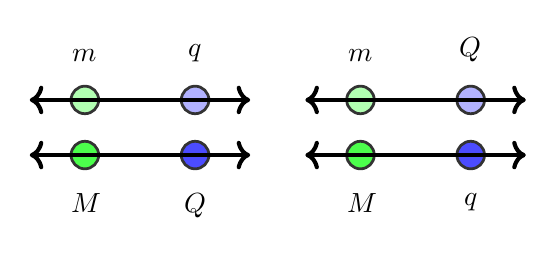
\begin{tikzpicture}[scale=0.7]
% \draw[step=0.5cm,gray!50,very thin] (-6,-6) grid (6,6);
% \draw[->,thin] (0,-6) -- (0,6);
% \draw[->,thin] (-6,0) -- (6,0);
% \draw (0,0) node[below] {$0$};
% \foreach \j in {-6, -5, ..., -1, 1, 2, ..., 6} {
%   \draw (\j,0) node[below=0.1]{\j};
%   \draw (0,\j) node[right=0.1]{\j};
% }

\coordinate (m) at (1,3);
\coordinate (q) at (3,3);
\coordinate (M) at (1,2);
\coordinate (Q) at (3,2);

\filldraw[fill=green!30, draw=black!80, line width=1pt] (m) circle (0.25cm) node[above=0.35cm] {$m$};
\filldraw[fill=blue!30, draw=black!80, line width=1pt] (q) circle (0.25cm) node[above=0.35cm] {$q$};
\filldraw[fill=green!70, draw=black!80, line width=1pt] (M) circle (0.25cm) node[below=0.35cm] {$M$};
\filldraw[fill=blue!70, draw=black!80, line width=1pt] (Q) circle (0.25cm) node[below=0.35cm] {$Q$};
\draw[<->,line width=1.5pt] ($(m)-(1,0)$)   -- ($(q)+(1,0)$);
\draw[<->,line width=1.5pt] ($(M)-(1,0)$)   -- ($(Q)+(1,0)$);


\coordinate (m) at (6,3);
\coordinate (Q) at (8,3);
\coordinate (M) at (6,2);
\coordinate (q) at (8,2);

\filldraw[fill=green!30, draw=black!80, line width=1pt] (m) circle (0.25cm) node[above=0.35cm] {$m$};
\filldraw[fill=blue!30, draw=black!80, line width=1pt] (Q) circle (0.25cm) node[above=0.35cm] {$Q$};
\filldraw[fill=green!70, draw=black!80, line width=1pt] (M) circle (0.25cm) node[below=0.35cm] {$M$};
\filldraw[fill=blue!70, draw=black!80, line width=1pt] (q) circle (0.25cm) node[below=0.35cm] {$q$};
\draw[<->,line width=1.5pt] ($(m)-(1,0)$)   -- ($(Q)+(1,0)$);
\draw[<->,line width=1.5pt] ($(M)-(1,0)$)   -- ($(q)+(1,0)$);

\end{tikzpicture}

\column{0.5\textwidth}

\begin{itemize}
\tightlist
\item
  Moleculars markers address the limitations of phenotypic markers
\item
  QTLs have greatest potential in Marker-Assisted Selection (MAS) for
  quantitatively inherited traits that have low heritability or that are
  difficult or expensive to screen or evaluate.
\end{itemize}

\ecolumns
\end{frame}

\begin{frame}{Types}
\protect\hypertarget{types}{}
\bcolumns
\column{0.6\textwidth}
\footnotesize

\begin{itemize}
\tightlist
\item
  Genomic markers, have particular strengths and weakness, so,
  consideration and knowledge of the markers is necessary before use.
\item
  For instance, a RAPD marker is dominant (identifying only one band of
  distinction) and it may be sensitive to reproducible results. This is
  typically due to the conditions in which it was produced. RAPD's are
  used also under the assumption that two samples share a same locus
  when a sample is produced.
\end{itemize}

\column{0.4\textwidth}

\begin{figure}
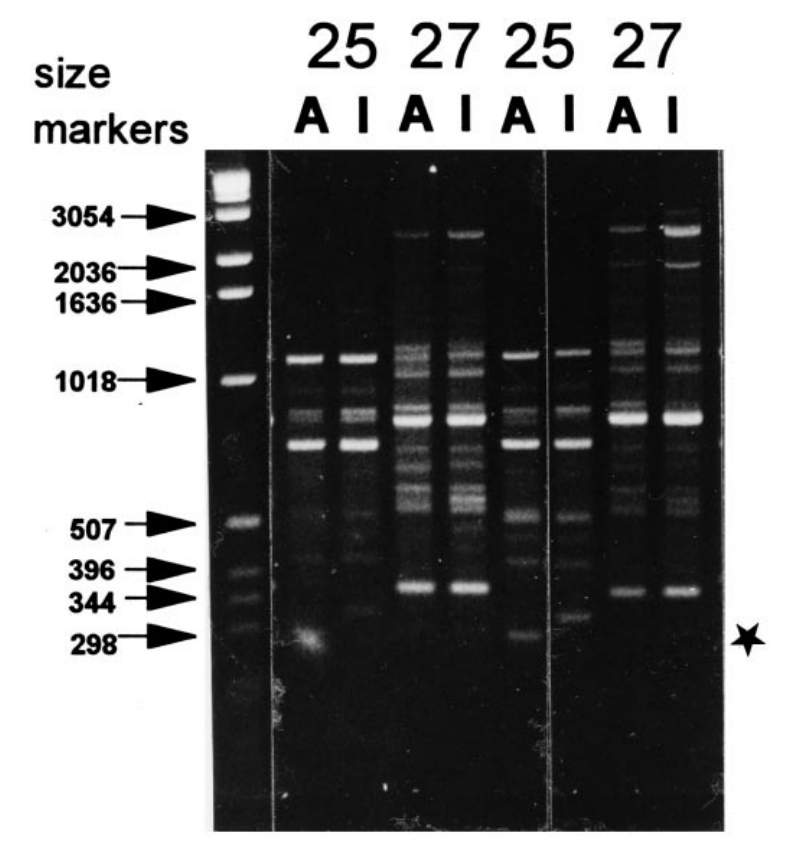
\includegraphics[width=0.5\linewidth]{../images/rapd_marker_diagram} \caption{The RAPD Genetic Screening Package. The RAPD profile as obtained by the package assembler Milan group (one of the participants of the study). Size markers for assessing base pair lengths are shown in the ladder of the far left track. Two profiles using primers FS-25 (given as 25) and FS-27 (given as 27) both of which are decamers are shown for the two cultivars Adige (A) and I-214 (I). The polymorphic bands observed with FS-25 are indicated by *. Source: \cite{jones1997reproducibility}}\label{fig:rapd-markers}
\end{figure}

\ecolumns
\end{frame}

\begin{frame}{}
\protect\hypertarget{section-2}{}
\bcolumns
\column{0.35\textwidth}
\footnotesize

\begin{itemize}
\tightlist
\item
  Commonly used molecular markers:

  \begin{itemize}
  \scriptsize
  \item Restriction Fragment Length Polymorphism -- RFLP
  \item Random Amplified Polymorphic DNA -- RAPD
  \item Amplified Fragment Length Polymorphism -- AFLP
  \item Variable Number Tandem Repeat -- VNTR
  \item Oligonucleotide Polymorphism -- OP
  \item Single Nucleotide Polymorphism -- SNP
  \item Allele Specific Associated Primers -- ASAP
  \item Inverse Sequence-tagged Repeats -- ISTR
  \end{itemize}
\end{itemize}

\column{0.65\textwidth}

\begin{table}

\caption{\label{tab:molecular-markers-distinction}A general comparison of molecular markers.}
\centering
\fontsize{4}{6}\selectfont
\begin{tabular}[t]{>{\raggedright\arraybackslash}p{8em}>{\raggedright\arraybackslash}p{6.5em}>{\raggedright\arraybackslash}p{6.5em}>{\raggedright\arraybackslash}p{6.5em}>{\raggedright\arraybackslash}p{6.5em}>{\raggedright\arraybackslash}p{6.5em}>{\raggedright\arraybackslash}p{6.5em}}
\toprule
Attribute & Isozyme & RFLP & RAPD & AFLP & SSR & SNP\\
\midrule
Abundance & Low & Medium & Very high & Very high & High & Very high\\
Types of polymorphism & Amino acid change in polypeptide & Single base change, indel, inversion & Single base change, indel, inversion & Single base change, indel, inversion & Repeat length variation & Single base change\\
DNA quality &  & High & Medium & High & Medium & Medium\\
DNA sequence information &  & Not required & Not required & Not required & Required & Required\\
Level of polymorphism & Low & Medium & High & High & High & High\\
Inheritance & Codominance & Codominance & Dominance & Dominance & Codominance & Codominance\\
Reproducibility & Medium & High & Low & Medium & High & Medium\\
Technical complexity & Medium & High & Low & Medium & Low & Medium\\
Developmental cost & Medium & High & Low & Low & High in the beginning & High\\
Transferability & High & Medium & High & High & Medium & Low\\
Automation & Low & Low & Medium & Medium & High & High\\
\bottomrule
\end{tabular}
\end{table}

\ecolumns
\end{frame}

\begin{frame}{}
\protect\hypertarget{section-3}{}
\begin{description}
\small
\item[Random-amplified polymorphic DNA (RAPDs)] involve the use of a single 'arbitrary' primer (purchasable from commercial companies) in a PCR reaction and result in the amplification of several discrete DNA products. Each product is derived from a region of the genome that contains two short segments in inverted orientation, on opposite strands, that are complementary to the primer and sufficiently close together for the amplification to work. In RAPDs, the amplification products are separated on agarose gels in the presence of ethidium bromide and visualised under ultraviolet light.
\item[Amplified fragment length polymorphism(AFLP)] is another PCR-based method which first involves restriction digestion of the genomic DNA. Adapters are ligated to the ends of the restricted fragments and either a pre-selection step performed using magnetic beads followed by a round of selective PCR, or two selective rounds of PCR amplification are applied. The amplified products are separated on a sequencing gel and can be visualised using radioactive or fluorescent labelling.
\end{description}
\end{frame}

\begin{frame}{Microsatellite (SSR) marker and genetic basis}
\protect\hypertarget{microsatellite-ssr-marker-and-genetic-basis}{}
\bcolumns
\column{0.4\textwidth}

\begin{figure}
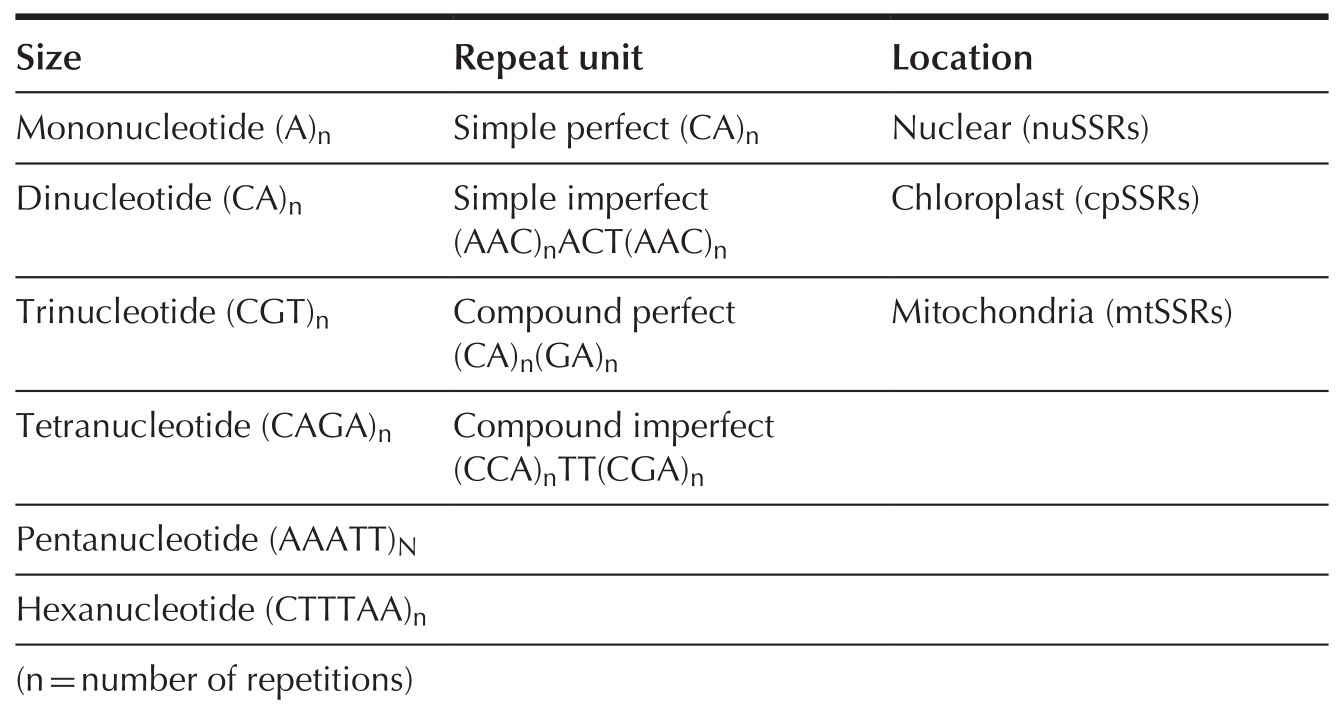
\includegraphics[width=0.95\linewidth]{../images/SSR_class} \caption{Types of microsatellite locus.}\label{fig:microsatellite-marker-classification}
\end{figure}

\column{0.6\textwidth}

\begin{figure}
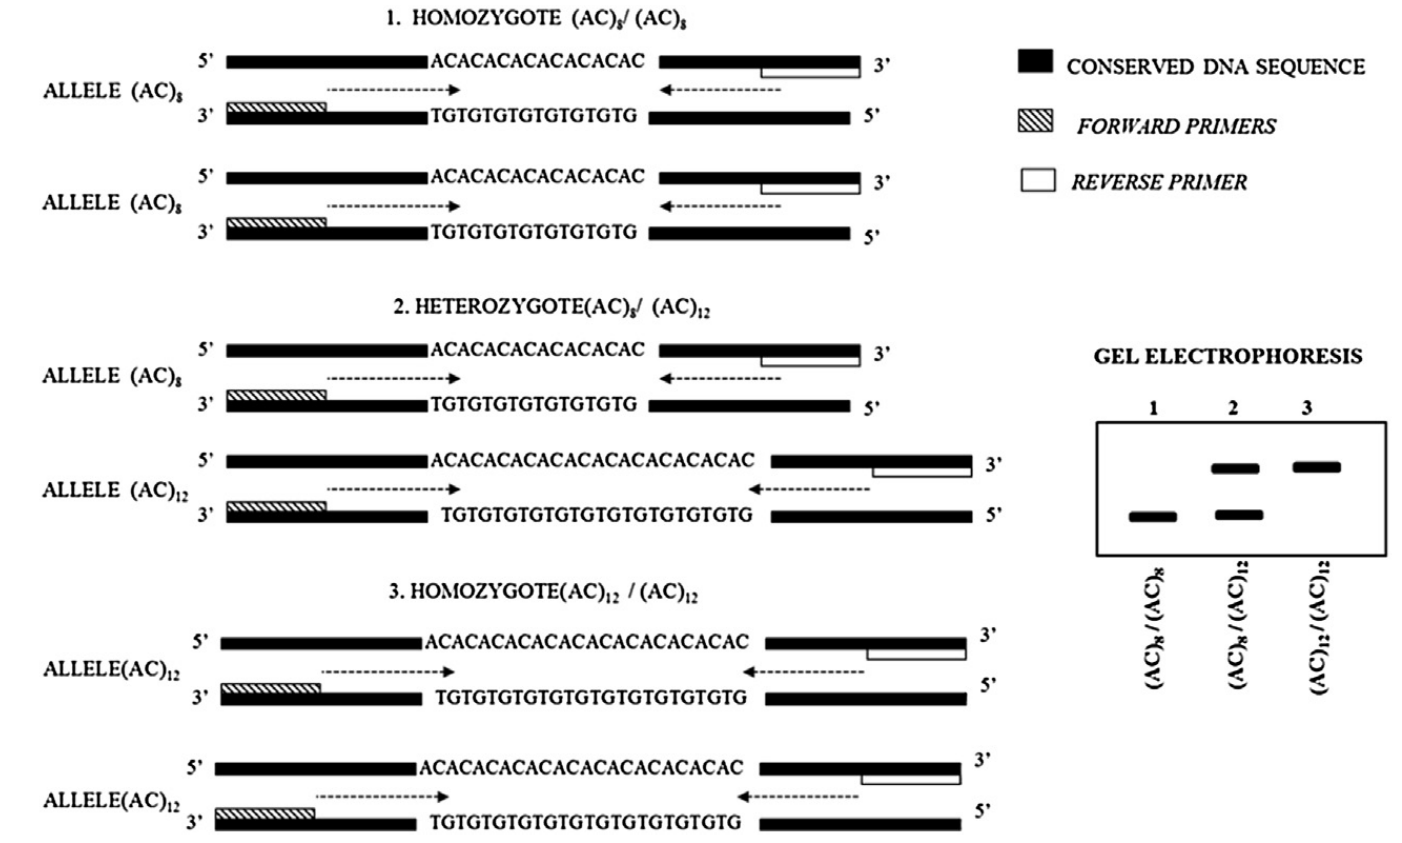
\includegraphics[width=0.98\linewidth]{../images/SSR_marker_genetic_basis} \caption{Genetic basis of microsatellite marker.}\label{fig:microsatellite-marker-basis}
\end{figure}

\ecolumns
\end{frame}

\begin{frame}{Applications}
\protect\hypertarget{applications}{}
\begin{itemize}
\tightlist
\item
  Assessing variability of genetic differences and characteristics
  within a species.
\item
  Identification and fingerprinting of genotypes.
\item
  Estimating genetic distances between species and offspring.
\item
  Identifying location of QTLs.
\item
  Identification of DNA sequence from useful candidate genes.
\end{itemize}
\end{frame}

\begin{frame}{Application of molecular marker: QTL mapping}
\protect\hypertarget{application-of-molecular-marker-qtl-mapping}{}
\footnotesize

\begin{itemize}
\tightlist
\item
  QTL mapping is based on idea that location of QTL in the genome can be
  identified using marker loci linked to a QTL.

  \begin{itemize}
  \tightlist
  \item
    Suppose you make a cross between two inbred strains -- P1 (with high
    trait value) and P2 (with low trait value).
  \item
    The F1 can be backcrossed to P1 to create a BC1 population in which
    the alleles at all the genes in the two parental genomes will
    segregate.
  \item
    Marker loci such as SNP or microsatellites can be scored
    unambiguously as homozygous P1 or heterozygous for each BC1
    individual.
  \item
    If there is a QTL linked to the marker locus, then the mean trait
    value for individuals that are homozygous P1 at the marker locus
    will be different from the mean trait value for the heterozygous
    individual.
  \item
    Contribution of the alleles to a QTL to the trait value can be
    observed by looking at the frequency distributions associated with
    each genotype at a QTL as shown in Figure
    \ref{fig:allele-freq-distribution}.
  \end{itemize}
\end{itemize}
\end{frame}

\begin{frame}{}
\protect\hypertarget{section-4}{}
\bcolumns
\column{0.55\textwidth}

\begin{figure}
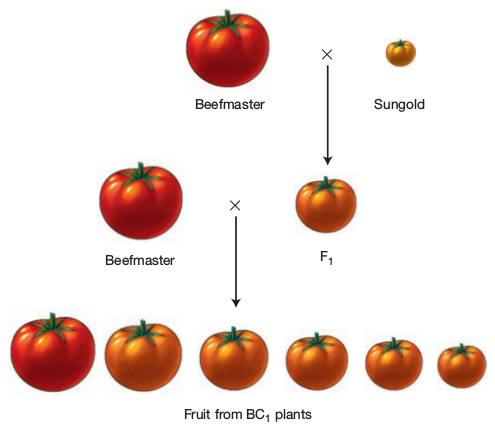
\includegraphics[width=0.72\linewidth]{../images/tomato-beefmaster-sungold-cross} \caption{Breeding scheme for a BC population between Beefmaster and Sunglod tomatoes. In the BC1 generation, there is a continuous range of fruit sizes.}\label{fig:tomato-beefmaster-sungold-cross}
\end{figure}

\column{0.45\textwidth}

\begin{figure}
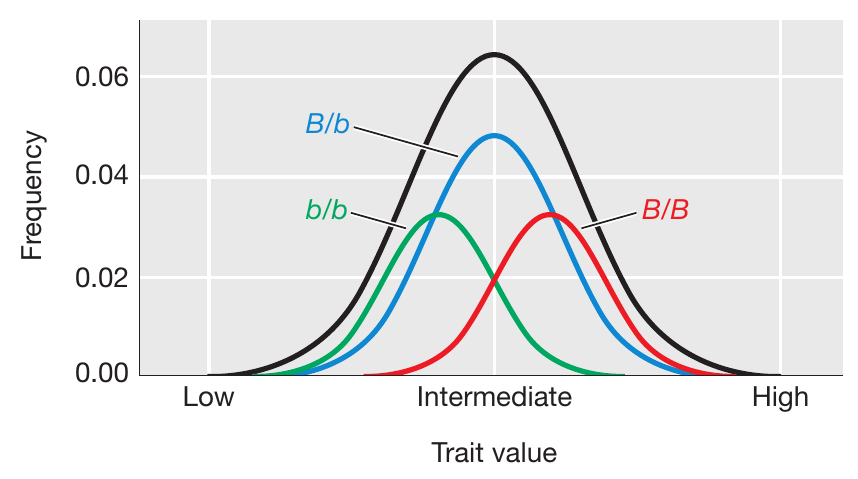
\includegraphics[width=0.92\linewidth]{../images/frequency_distribution_showing_contribution_qtl} \caption{Frequency distribution show the contributions of alleles at a QTL to a complex trait. Distributions for the different genotypic classes at QTL locus B relate to the overall distribution for the population (black lines)}\label{fig:allele-freq-distribution}
\end{figure}

\ecolumns
\end{frame}

\begin{frame}{}
\protect\hypertarget{section-5}{}
\begin{columns}[T,onlytextwidth]
  \column{0.4\textwidth}
  \begin{itemize}
  \footnotesize
  \item Let us take two inbred lines of tomato that differ in fruit weight -- Beefmaster with fruits of 230 g and Sungold with fruits of 10 g weights.
  \item Cross the two lines to produce F1, then backcross the F1 to the beefmaster line to produce BC1 generation.
  \item Several hundered BC1 plants are grown and their fruit weights measured.
  \item Extract DNA from each of the BC1 plants. These DNA samples are used to determine the genotype of each plant at a set of marker loci (SSRs) (~100)  that are distributed across all of the chromosomes such that we have marker locus every 5 to 10 centimorgans.
  \end{itemize}
  \column{0.6\textwidth}

\begin{figure}
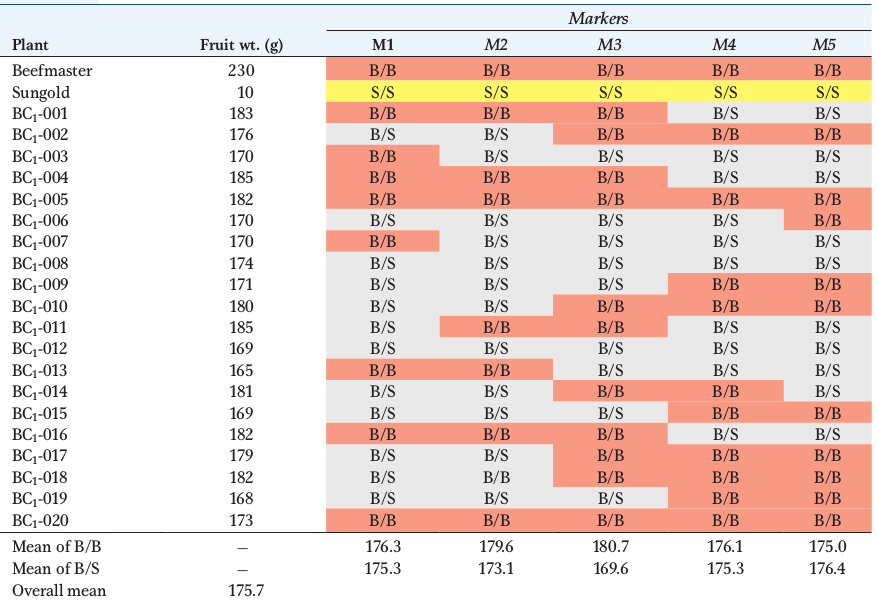
\includegraphics[width=0.95\linewidth]{../images/tomato-fruit-weight-marker-data} \caption{Example data of fruit weight and marker-locus data for BC population between inbred lines.}\label{fig:tomato-fruit-weight-marker-data}
\end{figure}

\end{columns}
\end{frame}

\begin{frame}{}
\protect\hypertarget{section-6}{}
\begin{itemize}
\tightlist
\item
  For each BC1 plant, we have the weight of its fruit and the genotypes
  at the marker loci. (Note: Trait values for the BC1 are intermediate
  between the two parents, but closer to the Beefmaster)
\item
  Since this is BC population, the genotypes at each marker locus is
  either B/B or B/S.
\item
  Crossover results in two markers appearing in recombinant/non-parental
  alignments (eg, BC1-001 has crossover between marker loci M3 and M4).
\item
  The expectation is that there is no QTL affecting fruit weight near M1
  -- For M1, the mean for genotypic classes B/B is 176.3 adn that for
  B/S is 175.3 (both lying close to overall mean 175.7). Now determine
  that for M3 ?
\item
  For M3, it matches the expectation that there is a QTL affecting fruit
  weight near M3.
\end{itemize}
\end{frame}

\begin{frame}{Requirements of QTL mapping}
\protect\hypertarget{requirements-of-qtl-mapping}{}
\begin{itemize}
\tightlist
\item
  Breeding facilities with environmental control, accurate phenotyping
  and trained manpower
\item
  Incomplete linkage between a marker and the target QTL reduces the
  effectiveness of MAS
\item
  Marker must be polymorphic on the parents
\item
  MAS is effective only if the alleles being selected are important
  relative to other alleles in the population; For example a breeder
  might identify that allele A1 at locus A has a positive effect on
  yield. But this prediction would be made in a limited set of
  environments, and with a limited set of germplasm. A breeder who
  crossed a parent containing allele A1 with a new parent containing
  allele A4, and selected for A1 using a linked marker, might never
  discover that A4 is actually better than allele A1, or perhaps that
  allele A1 causes plants to be susceptible to a disease that was not
  present when A1 was first characterized. Hence, MAS should never to
  applied independently of phenotypic selection.
\end{itemize}
\end{frame}

\begin{frame}{Factors affecting QTL mapping using biparental
populations}
\protect\hypertarget{factors-affecting-qtl-mapping-using-biparental-populations}{}
\begin{enumerate}
\tightlist
\item
  Size of mapping population
\item
  Nature of mapping populations
\item
  Density and coverage of markers in the linkage map
\item
  Statistical methods used
\item
  Heritability of the trait
\item
  Significance criteria used
\item
  Effect of environment
\item
  Experimental errors
\end{enumerate}
\end{frame}

\hypertarget{marker-assisted-selection}{%
\section{Marker assisted selection}\label{marker-assisted-selection}}

\begin{frame}{}
\protect\hypertarget{section-7}{}
\begin{itemize}
\tightlist
\item
  Individual genes contributing to complex plant traits can sometimes be
  discovered through their association with genetic markers --
  \alert{QTL analysis}.
\item
  Use of molecular markers in detecting regions of genome and
  discriminating between genotypes based on genomic features that
  enhance chances of inheriting favorable quantitative trait loci is
  called MAS.
\item
  Rather than selecting traits, which are outcome of many genes, MAS is
  based on selecting specific alleles at marker loci that are known to
  be linked to the genes that cause the desired trait.
\end{itemize}
\end{frame}

\begin{frame}{Requirements}
\protect\hypertarget{requirements}{}
\begin{itemize}
\tightlist
\item
  Marker should co-segregate or map as close as possible to the target
  gene (e.g.~less than 2cM), in order to have low recombination
  frequency between the target gene and the marker.
\end{itemize}

\begin{itemize}
\tightlist
\item
  For unlimited use in MAS, markers should display polymorphism between
  genotypes that have and do not have the target gene.
\item
  Cost-effective, simple and high-throughput markers are required to
  ensure genotyping power needed for the rapid screening of large
  populations.
\end{itemize}

\begin{itemize}
\tightlist
\item
  Marker-assisted background selection depends on molecular markers that
  are well characterized and distributed over the whole genome.
\end{itemize}
\end{frame}

\begin{frame}{Advantages}
\protect\hypertarget{advantages}{}
\begin{enumerate}
\tightlist
\item
  Avoids errors caused by environmental variance
\item
  Can be applied at a juvenile stage before a trait is expressed
\item
  Can be applied on a single plant
\item
  May be less expensive than phenotypic selection (it is debatable!)
\end{enumerate}

\begin{figure}
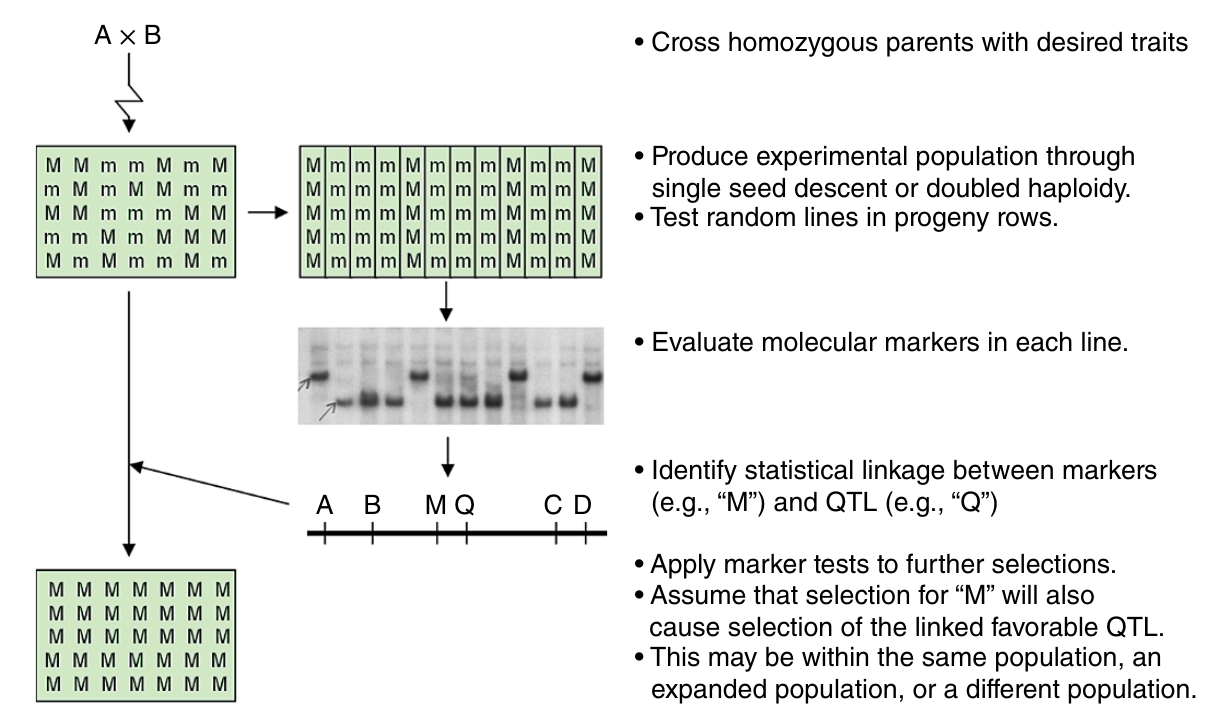
\includegraphics[width=0.38\linewidth]{../images/marker_assisted_selection} \caption{A simplified strategy for MAS. Here, a significant association between a QTL (Q) and a molecular marker allele (M) is identified in an experimental population. This information is applied in future populations in order to select Q indirectly through its linkage to M.}\label{fig:marker-assisted-selection}
\end{figure}
\end{frame}

\begin{frame}{MAS: A simulated case study}
\protect\hypertarget{mas-a-simulated-case-study}{}
\footnotesize

\begin{itemize}
\tightlist
\item
  Two homozygous parents are hybridized to produce \(\mathrm{F_1}\)
  plants. One parent was homozygous
  AABBCC\footnote[frame]{Note that A is not dominant to a, etc.} at the
  A-, B- and C-bands (molecular bands), respectively, while the other
  parent was homozygous aabbcc.

  \begin{itemize}
  \footnotesize
  \item 32 homozygous lines were derived from $\mathrm{F_1}$ using DH techniques.
  \item all lines were grown in 4 replicated field trial to determine yield of each
  \item lines are polymorphic for 3 loci that appeared to be located on the same chromosome
  \end{itemize}
\end{itemize}
\end{frame}

\begin{frame}{}
\protect\hypertarget{section-8}{}
\renewcommand{\arraystretch}{0.8}

\begin{table}

\caption{\label{tab:marker-phenotype-data}Yield of 32 double haploid canola lines, and genotype of each line at the A-, B-, and C- loci.}
\centering
\fontsize{5}{7}\selectfont
\begin{tabular}[t]{rlllr}
\toprule
Line & A-loci & B-loci & C-loci & Yield\\
\midrule
1 & AA & BB & CC & 108\\
2 & AA & BB & CC & 114\\
3 & AA & BB & cc & 112\\
4 & aa & bb & CC & 101\\
5 & aa & bb & cc & 91\\
6 & aa & bb & cc & 112\\
7 & aa & bb & cc & 97\\
8 & aa & bb & cc & 96\\
9 & aa & BB & CC & 114\\
10 & aa & BB & CC & 119\\
11 & AA & bb & cc & 98\\
12 & AA & BB & CC & 107\\
13 & AA & BB & CC & 118\\
14 & AA & BB & CC & 113\\
15 & AA & bb & CC & 102\\
16 & aa & BB & CC & 119\\
17 & aa & BB & cc & 112\\
18 & aa & bb & cc & 105\\
19 & aa & bb & cc & 105\\
20 & AA & BB & CC & 115\\
21 & AA & BB & CC & 111\\
22 & AA & bb & cc & 101\\
23 & AA & BB & cc & 117\\
24 & aa & bb & CC & 102\\
25 & aa & bb & cc & 106\\
26 & aa & bb & cc & 95\\
27 & AA & BB & CC & 122\\
28 & AA & BB & CC & 112\\
29 & AA & bb & cc & 105\\
30 & AA & bb & cc & 99\\
31 & aa & BB & CC & 116\\
32 & aa & bb & cc & 100\\
\bottomrule
\end{tabular}
\end{table}
\end{frame}

\begin{frame}{}
\protect\hypertarget{section-9}{}
\bcolumns
\column{0.6\textwidth}
\small

\begin{itemize}
\tightlist
\item
  Steps in QTL analysis

  \begin{enumerate}
  \footnotesize
  \item Determine whether there are indeed significant differences between the progeny lines -- accomplished by Analysis of Variance.
  \item Can significant differences in yield detected between the parental lines be explained by association between yield and the single marker bands ?
    \begin{itemize}
    \footnotesize
    \item average yield of each single band genotype can be calculated by adding the yield of lines carrying the same bands at each locus and dividing by the number of individual lines in that class
    \item there appears to be a pattern that lines carrying $AA$ band rather than $aa$, lines carrying $BB$ rather than $bb$ and lines carrying $CC$ band rather than $cc$ have an advantage in yield.
    \end{itemize}
  \end{enumerate}
\end{itemize}

\column{0.4\textwidth}

\renewcommand{\arraystretch}{1}

\begin{table}

\caption{\label{tab:marker-phenotype-data-summary}Average yield of each band genotype}
\centering
\fontsize{6}{8}\selectfont
\begin{tabular}[t]{lr}
\toprule
Genotype & Yield\\
\midrule
aa & 106\\
AA & 110\\
bb & 101\\
BB & 114\\
cc & 103\\
\addlinespace
CC & 112\\
\bottomrule
\end{tabular}
\end{table}

\ecolumns
\end{frame}

\begin{frame}{}
\protect\hypertarget{section-10}{}
\begin{figure}
  \begin{columns}[T,onlytextwidth]

  \column{.6\linewidth}
  \begin{center}
  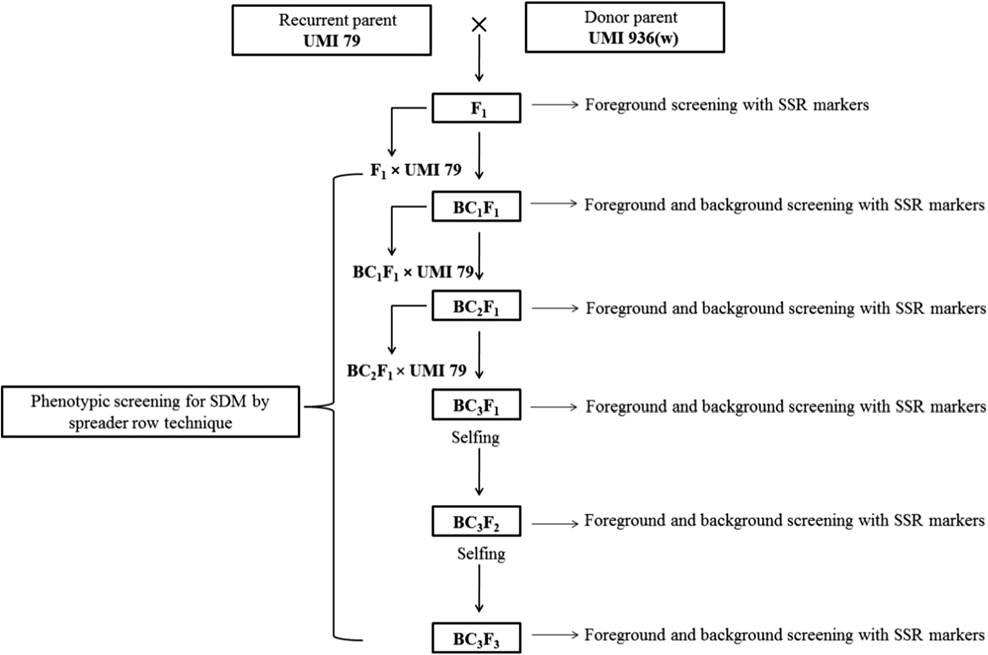
\includegraphics[width=0.94\linewidth]{../images/sorghum_backcross_breeding_marker_assisted.png}
  \end{center}
  
  \column{.4\linewidth}
  \caption{\newline An overview on improvement of sorghum downy (\textit{Peronosclerospora sorghi}) mildew resistance of Maize by marker-assisted back crossing (MABC). Two QTLs for SDM on Chromosome 3 and 6 from UMI 936 (w) were transferred into an elite maize inbred line UMI-79. For foreground selection, plants carrying heterozygous allele for the QTLs for SDM were selected from F1 and three backcross (BC1-BC3) generations using SSR markers linked to the targeted QTL region of SDM. Consequently foreground positive plants from BC3F1 generation selfed to produce BC3F2 and plants carrying the favorable alleles for the QTLs for SDM were selected followed by stringent phenotyping against SDM and advanced to BC3F3. As a result, two improved lines (79/936-1-7-7-7-46-46 and 79/936-1-7-7-10-80-80) possessing QTLs for SDM were obtained. Background selection using 146 SSR markers distributed evenly across maize genome revealed 92.45\% and 89.68\% recovery of recurrent parent genome in two improved lines. Phenotypic characterization showed more than 90\% recovery of the parents in morphological traits and resistance to SDM. Source: \cite{sumathi2020introgression}}
  \label{fig:sorghum-mas}
  
  \end{columns}
\end{figure}
\end{frame}

\begin{frame}{Progress in MAS}
\protect\hypertarget{progress-in-mas}{}
\begin{itemize}
\tightlist
\item
  It is now possible to select across a genome rather than select for
  one or several markers for single QTLs. Genomic selection is an
  extension of MAS.
\item
  In soybean, 50,000 single nucleotide polymorphic (SNP) markers are now
  available for use by breeders.
\end{itemize}
\end{frame}

\hypertarget{bibliography}{%
\section{Bibliography}\label{bibliography}}

\begin{frame}{See also}
\protect\hypertarget{see-also}{}
\begin{itemize}
\tightlist
\item
  Refer to Chapter 4 on ``Marker-assisted selection as a component of
  conventional plant breeding'', Plant breeding reviews, Volume 33.
\item
  Refer to Chapter 12 on ``Marker-assisted selection'', Plant Breeding
  Reviews, Volume 24, Part 1.
\end{itemize}
\end{frame}

\begin{frame}{References}
\protect\hypertarget{references}{}
\end{frame}

\begin{frame}[allowframebreaks]{}
  \bibliographytrue
  \bibliography{../bibliography/bibliographies.bib}
\end{frame}

\end{document}
